\documentclass[11pt,a4paper]{article}
\usepackage[margin=1in]{geometry}
\usepackage{amsmath,amssymb}
\usepackage{booktabs}
\usepackage{graphicx}
\usepackage{hyperref}
\usepackage{authblk}
\usepackage[T1]{fontenc}
\usepackage{tikz}
\usetikzlibrary{arrows.meta,positioning}
\usepackage{caption}
\captionsetup[figure]{name=Fig.,labelfont=bf,labelsep=space}

\title{AWS Cloud Security Detection: A Comparative Evaluation of Rule-Based and Machine Learning Methods}

\author[1]{Bisma Nadeem\thanks{Corresponding author. ORCID: to be added upon submission.}}
\author[1]{Noor-ul-Ain}
\affil[1]{Independent Researcher, Lahore, Pakistan (B.S. Computer Science, PUCIT, University of the Punjab, 2024). Email: bismanadeempucit@gmail.com, noorulain.pucit@gmail.com}

\date{}

\begin{document}
\maketitle

\begin{abstract}
\textbf{Purpose}: IAM misconfigurations are a leading cause of cloud security incidents. This study tests whether feature-engineered classifiers detect AWS risks more reliably than rule-based scanners across three tasks, IAM misconfiguration, API misuse, and CloudTrail anomalies, and whether any advantage survives contact with real data and an adversarial attacker.

\textbf{Methods}: For each task we compared a rule-based or feature-engineered baseline against a trained classifier (Random Forest for IAM and API misuse, Isolation Forest for CloudTrail) on synthetic but structurally realistic data. The IAM detector was also tested, without retraining, against 19 real, live AWS-managed IAM policies. The API misuse detector was tested against an attacker spreading sensitive calls thinly across a session to evade burst detection.

\textbf{Results}: Random Forest reached 98.3\% accuracy on synthetic IAM detection versus 75.0\% for the rule-based scanner, and 99.4\% accuracy with 100\% recall on API misuse. Against real policies, the same IAM model collapsed to 42.1\% accuracy, worse than the rule-based scanner's 84.2\%, because one feature overfit the synthetic vocabulary; generalizing it recovered accuracy to 84.2\% and recall to 87.5\%. Against the adversarial attacker, recall collapsed from 100\% to 3.0\%; widening the window alone did not help, and only training on evasive examples restored 100\% recall. Isolation Forest reached 97.4\% recall on CloudTrail anomalies.

\textbf{Conclusion}: Feature-engineered classifiers can substantially outperform rule-based baselines, but that advantage does not automatically generalize to real data or to an adversary evading the trained pattern. Both failures were visible only by testing outside the model's original conditions, and both were fixable once identified. Code, data, and results are publicly available.
\end{abstract}

\noindent\textbf{Keywords} Cloud security, Identity and Access Management, AWS, Machine learning, Anomaly detection, Adversarial evaluation

\section{Introduction}

Most cloud security incidents don't start with a zero-day. They start with something boring: an IAM role with \texttt{s3:*} on \texttt{Resource: *} that nobody meant to leave that broad, or a service account that was supposed to be scoped to one S3 bucket and somehow ended up with \texttt{AssumeRole} rights on three others. Reports on cloud breaches consistently point to human error and misconfiguration as leading causes rather than novel exploits, Thales' 2024 Cloud Security Study, for instance, found misconfiguration and human error behind 31\% of reported cloud breaches that year \cite{thales2024}.

The complication is scale. A small AWS account might have a dozen IAM roles. A mid-sized organization can easily have thousands of policies, spread across accounts, changing weekly as CI/CD pipelines create and modify roles automatically. At that point, a human reviewing policies one at a time is not a realistic security control.

This is the part of the problem we wanted to actually work through rather than just describe: what does automated detection catch, what does it miss, and where specifically does moving from a hand-written rule to a trained model help. We picked three specific, bounded tasks that map to real day-to-day cloud security work:

\begin{enumerate}
\item \textbf{IAM policy review}: flagging risky permissions in a set of policy documents.
\item \textbf{API behavior monitoring}. Spotting sessions where the sequence of API calls looks like reconnaissance or misuse rather than normal operation.
\item \textbf{CloudTrail log triage}, picking the small fraction of events in a large log stream worth a human looking at.
\end{enumerate}

For each, we compare a simple baseline against a trained model on the same data, and report where the gap actually is. And, for Experiment 1, whether that gap survives contact with real data.

\section{Related Work}

Static analysis of IAM policies is an established approach. Shevrin et al.\ build a formal model-checking approach that treats AWS IAM as a finite-state system and searches for privilege-escalation paths that a syntactic scanner would miss, evaluating it against real AWS environments containing hundreds of resources \cite{shevrin2023}. Van Ede et al.\ take a related angle, learning to flag anomalous IAM configurations from observed policy structure rather than a fixed rule set \cite{vanede2022}. More recently, Wen et al.\ explore using large language models directly as the detection mechanism for serverless misconfigurations \cite{wen2024}, a different tradeoff (no training data needed, but less controllable and harder to explain a specific flag). Misconfiguration detection is not unique to IAM: Rahman et al.\ run a comparable empirical study on Kubernetes manifests, finding that a large fraction of real-world open-source manifests contain at least one exploitable misconfiguration despite the availability of static scanners \cite{rahman2023}, the same practical gap between ``a rule exists'' and ``the rule catches what matters'' that motivates this paper's IAM experiment.

On the response side, several recent papers explore reinforcement learning for automating the mitigation step once something is flagged \cite{rlsecurity2025,rlincident2025}. We don't implement an RL response layer here: it is listed under future work. But these approaches report the same practical tension we ran into with static rules: overly aggressive automated response causes its own disruption, so reward/policy design has to weigh false-positive cost, not just detection rate.

For grounding the practical scale of the problem, industry reporting is more useful than academic benchmarks, since very little labeled real-world breach data is published for privacy reasons. The Cloud Security Alliance's 2024 Top Threats survey, based on responses from over 500 industry security professionals, ranks misconfiguration/change control and IAM weaknesses as the two most significant cloud security concerns \cite{csa2024}. NIST's Zero Trust architecture guidance \cite{nist800207} and OWASP's API Security Top 10 \cite{owasp2023} both treat least-privilege enforcement and behavioral monitoring as baseline expectations rather than advanced measures, which matches what we saw building even this small-scale version of the problem.

\section{Methodology}

All three experiments follow the same shape: generate a synthetic dataset with realistic structure (including deliberately ambiguous cases), run a simple baseline detector, then train a classifier on engineered features and compare. Experiment 1 goes one step further and is also checked against real, external data (Section 3.1).

There is no publicly available, labeled dataset of real AWS IAM policies or CloudTrail logs, for good reason, since that data is sensitive by nature. Building a synthetic generator is the standard workaround in this space; a similarly-motivated synthetic IAM/API dataset has been published on IEEE DataPort for the same reason \cite{ieeedataport}. The value of a synthetic experiment isn't ``this exact accuracy number will hold in production'', it's demonstrating where a detection approach structurally succeeds or fails, using data where we control and know the ground truth. Where possible (Experiment 1), we then check whether that structural conclusion survives contact with data we don't control.

Figure~\ref{fig:pipeline} summarizes the overall pipeline shared across the three experiments, and shows where the Experiment~1 external-validation path (Section 3.1) departs from the synthetic-only path used in Experiments 2 and 3.

\begin{figure}[h]
\centering
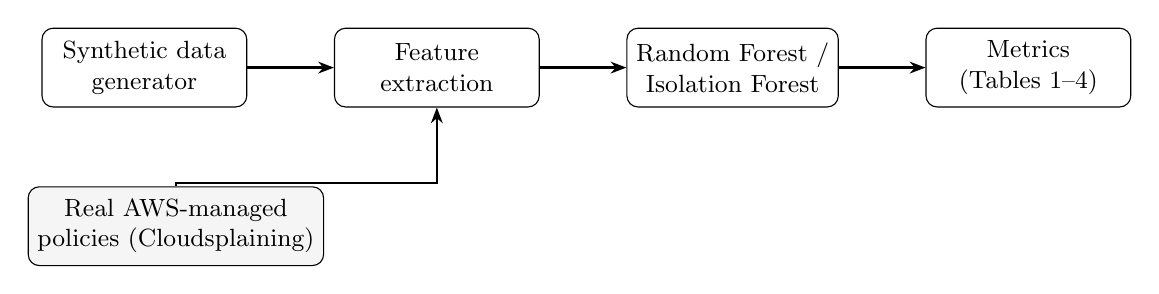
\begin{tikzpicture}[
  box/.style={draw, rounded corners, align=center, minimum height=1cm, minimum width=2.6cm, font=\small},
  arr/.style={-{Stealth[length=2mm]}, thick}
]
\node[box] (synth) {Synthetic data\\generator};
\node[box, right=1.1cm of synth] (feat) {Feature\\extraction};
\node[box, right=1.1cm of feat] (model) {Random Forest /\\Isolation Forest};
\node[box, right=1.1cm of model] (metrics) {Metrics\\(Tables 1--4)};

\node[box, below=1.0cm of synth, xshift=0.4cm, fill=gray!8] (real) {Real AWS-managed\\policies (Cloudsplaining)};

\draw[arr] (synth) -- (feat);
\draw[arr] (feat) -- (model);
\draw[arr] (model) -- (metrics);
\draw[arr] (real) -- ++(0,0.55) -| (feat.south);
\end{tikzpicture}
\caption{Shared experiment pipeline. Solid top row: synthetic-data path used in all three experiments (train and test). Bottom node: the external-validation path used only in Experiment~1, where real AWS-managed policy documents are passed through the same, unmodified feature extractor as an out-of-distribution test set for a model trained purely on synthetic data}
\label{fig:pipeline}
\end{figure}

\subsection{Experiment 1: IAM Misconfiguration Detection}

We generated 200 synthetic IAM policy documents across three categories: safe (120), risky (50), and critical/wildcard (30). To avoid the trivial version of this problem, we added two deliberately ambiguous cases: about 15\% of ``safe'' policies carry a low-visibility risky action tucked into a second statement, and about 10\% of ``risky'' policies use a legitimate two-statement pattern (\texttt{iam:PassRole} + \texttt{sts:AssumeRole} scoped to a CI/CD deployment role) that is structurally identical to a privilege-escalation pattern but is actually a normal, safe configuration in many real deployments.

The rule-based detector flags any statement containing a wildcard action or wildcard resource. The ML detector is a Random Forest trained on seven engineered features aggregated across all statements in a policy: statement count, total action count, presence of wildcard action/resource, count of known-risky actions, count of known-dangerous actions, and a binary flag for the PassRole+AssumeRole combination.

\paragraph{External validation on real, live AWS-managed policies.} Training and testing on our own synthetic generator risks a circularity problem: we define what ``risky'' looks like, then check whether a model can learn our own definition. To get outside that loop, we additionally evaluate both detectors. Trained only on synthetic data, against 30 real IAM policy documents that are not synthetic and not written by us: the actual, currently-published JSON policy documents behind AWS's own managed policies (\texttt{arn:aws:iam::aws:policy/...}, e.g.\ \texttt{AdministratorAccess}, \texttt{AmazonS3ReadOnlyAccess}, \texttt{AmazonEC2FullAccess}), obtained from the Apache-2.0-licensed test corpus of Cloudsplaining, an open-source AWS IAM security scanner \cite{cloudsplaining}, which mirrors real \texttt{iam:GetAccountAuthorizationDetails} output. Ground truth for this external set follows AWS's own published IAM best-practice guidance rather than anything we invented: a policy is labeled ``broad/risky'' if its name ends in \texttt{FullAccess} or is \texttt{AdministratorAccess}/\texttt{PowerUserAccess}, and ``narrow/safe'' if it ends in \texttt{ReadOnlyAccess}/\texttt{ViewOnlyAccess}. 19 of the 30 policies fall unambiguously into one of these two buckets by name; the remaining 11 are excluded from the labeled comparison rather than force-labeled.

\subsection{Experiment 2: API Misuse Detection}

We generated 1{,}000 ``normal'' API call sessions and 200 ``malicious'' sessions (8--20 calls each), where malicious sessions cluster sensitive calls (\texttt{ListUsers}, \texttt{DeleteRole}, \texttt{PutPolicy}, \texttt{CreateAccessKey}, \texttt{AttachUserPolicy}, \texttt{AssumeRole}) into a short burst. We also added noisy normal sessions (8\% of the normal set) with one isolated sensitive call and no burst pattern.

We engineered six features per session: session length, sensitive-call count and ratio, unique-action ratio, maximum sensitive-call burst in any 4-call sliding window, and repeated-bigram frequency. A Random Forest was trained on these features.

To move past a purely hypothetical limitation, we ran an actual adversarial evaluation. We generated 200 independently-seeded ``low-and-slow'' sessions. An attacker spreading 6 sensitive calls across a 50-call session, spaced so no 4-call window ever contains more than 1--2 of them, and measured detection. We then tested two candidate fixes against the same held-out adversarial sessions: (a) adding burst features at wider windows ($w=4,10,20$) without changing the training data, and (b) additionally training on a small, disjoint set of low-and-slow examples (100 sessions, different random seeds from the 200 held-out evaluation sessions, so there is no train/test leakage).

\subsection{Experiment 3: CloudTrail Anomaly Detection}

We generated 50{,}000 synthetic CloudTrail-style events, 1{,}500 of them (3\%) anomalous. Normal events cluster around business hours, use common event names and regions, and have a low error rate. Anomalous events are shifted toward off-hours activity, rare event names/regions, higher error rates, and higher call rate.

We used an Isolation Forest, given the true contamination rate (3\%), on five features: hour of day, event rarity flag, region rarity flag, error flag, and calls-per-minute.

\paragraph{External grounding check (not a full real-data test).} Unlike Experiment 1, we could not obtain a public, labeled, real-world CloudTrail dataset for this project, real CloudTrail logs are sensitive by nature, and the one known public raw-log dataset from a deliberately-vulnerable environment is a large binary archive not practical to obtain and parse here (noted as future work, Section 7). What we could do: check whether our synthetic generator's notion of a ``rare/sensitive'' event name is grounded in anything real, by cross-referencing our six rare-event names against TrailDiscover, an open-source, incident-report-linked catalog of 381 CloudTrail event names with a \texttt{usedInWild} flag sourced from published security incident write-ups \cite{traildiscover}. The result is a genuine limitation, not a confirmation: only 2 of our 6 ``rare'' event names (\texttt{DeleteTrail}, \texttt{CreateAccessKey}) are currently documented there as used in a real, publicly written-up attack, while 3 of our 7 ``common'' event names (\texttt{GetObject}, \texttt{ListBuckets}, \texttt{PutLogEvents}) are \emph{also} documented as attacker-abused. Rarity of an event name by itself is a weaker real-world signal than the generator assumes; we report this directly as a limitation (Section 6) rather than rebuilding Experiment 3 around it.

\section{Results}

\subsection{Experiment 1}

\begin{table}[h]
\centering
\begin{tabular}{@{}lccc@{}}
\toprule
Detector & Accuracy & Precision & Recall \\
\midrule
Rule-based (wildcard scan) & 75.0\% & 100\% & 37.5\% \\
Random Forest & 98.3\% & 100\% & 95.8\% \\
\bottomrule
\end{tabular}
\caption{Standard synthetic held-out test set.}
\end{table}

The rule-based scanner has perfect precision but low recall, because it structurally cannot see the cross-statement PassRole+AssumeRole pattern. The Random Forest, working from features that aggregate across the whole policy, closes almost all of that gap, matching what the model-checking literature has already argued for real AWS environments \cite{shevrin2023}.

\paragraph{External validation on real AWS-managed policies.} This is the more important table in this section (Table 2). The numbers above are on synthetic data the model was, in effect, designed to succeed on.

\begin{table}[h]
\centering
\begin{tabular}{@{}lcc@{}}
\toprule
Detector & Real-data accuracy & Real-data recall \\
\midrule
Rule-based (wildcard scan) & 84.2\% & 100\% \\
Random Forest (original features) & 42.1\% & 37.5\% \\
Random Forest (generalized wildcard feature) & 84.2\% & 87.5\% \\
\bottomrule
\end{tabular}
\caption{External test: 19 real, live AWS-managed IAM policies (not synthetic).}
\end{table}

The rule-based scanner transfers \emph{better} than the original Random Forest here (84.2\% vs.\ 42.1\% accuracy): the opposite ranking from Table 1. The reason is mechanistic and traceable: the original \texttt{num\_dangerous\_actions} feature checks for three literal strings (\texttt{*}, \texttt{iam:*}, \texttt{s3:*}), exactly the set our synthetic generator happened to use. Real AWS-managed policies use dozens of other service-level wildcards (\texttt{ec2:*}, \texttt{rds:*}, \texttt{route53:*}, ...) this feature was blind to, so the model systematically under-flagged real risky policies like \texttt{AmazonEC2FullAccess} and \texttt{AmazonRoute53FullAccess}. Replacing that one feature with a general ``action is \texttt{*} or ends in \texttt{:*}'' pattern match recovers accuracy to 84.2\% and recall to 87.5\%, matching the rule-based scanner on accuracy while beating it on recall, without any change to Table 1's synthetic-data numbers. A classifier's apparent advantage over a simpler baseline can be an artifact of how narrowly its features were defined relative to its training distribution. Visible only by testing outside that distribution.

\subsection{Experiment 2}

\begin{table}[h]
\centering
\begin{tabular}{@{}lc@{}}
\toprule
Metric & Value \\
\midrule
Accuracy & 99.4\% \\
Precision & 96.2\% \\
Recall & 100\% \\
False positive rate & 0.74\% \\
\bottomrule
\end{tabular}
\caption{Experiment 2, standard held-out test set.}
\end{table}

Every actual malicious session in the standard test set was caught; remaining error is entirely false positives from noisy ``legitimate isolated sensitive call'' sessions.

\paragraph{Adversarial evaluation (low-and-slow attacker).} Against 200 held-out low-and-slow sessions, the baseline $w{=}4$ detector caught 6 out of 200 (3.0\% recall). Adding wider burst windows ($w=4,10,20$) \emph{without} retraining on spread-out examples did not help: recall stayed at exactly 3.0\%. The fix only works once the model is trained on some low-and-slow examples, with 100 such sessions added to training (disjoint seeds from evaluation), recall on the held-out adversarial set rose to 100\%, and standard-test accuracy \emph{improved slightly} (99.71\% vs.\ 99.38\%), with false-positive rate dropping from 0.74\% to 0.37\%.

\begin{table}[h]
\centering
\begin{tabular}{@{}lcc@{}}
\toprule
Model & Standard test recall & Low-and-slow adversarial recall \\
\midrule
Baseline ($w=4$), no adversarial training & 100\% & 3.0\% \\
Multi-window ($w=4,10,20$), no adversarial training & 100\% & 3.0\% \\
Multi-window + adversarial training & 100\% & 100\% \\
\bottomrule
\end{tabular}
\caption{Adversarial evaluation: standard vs.\ low-and-slow recall across model variants.}
\end{table}

Wider windows alone did nothing; what closed the gap was training on examples of the evasive behavior. The reported 100\% post-fix recall is specific to the one evasion strategy tested and should not be read as general adversarial robustness.

Table 3 tests a single window size ($w=4$) against its two natural alternatives. To check that this isn't an artifact of that one specific window choice, we swept the burst-detection window size itself across $w \in \{4,6,8,10,15,20,30,40\}$, retraining and re-evaluating a fresh model at each value (Figure~\ref{fig:sweep}). The pattern holds at every window size tested, not just $w=4$: without adversarial training, low-and-slow recall stays at 0--3\% regardless of how wide the window is; with adversarial training, it is 100\% at every window size. Standard-test recall degrades mildly as the window widens (100\% down to 90\%), a real, if minor, cost of over-widening the window that Table 3 alone does not show.

\begin{figure}[h]
\centering
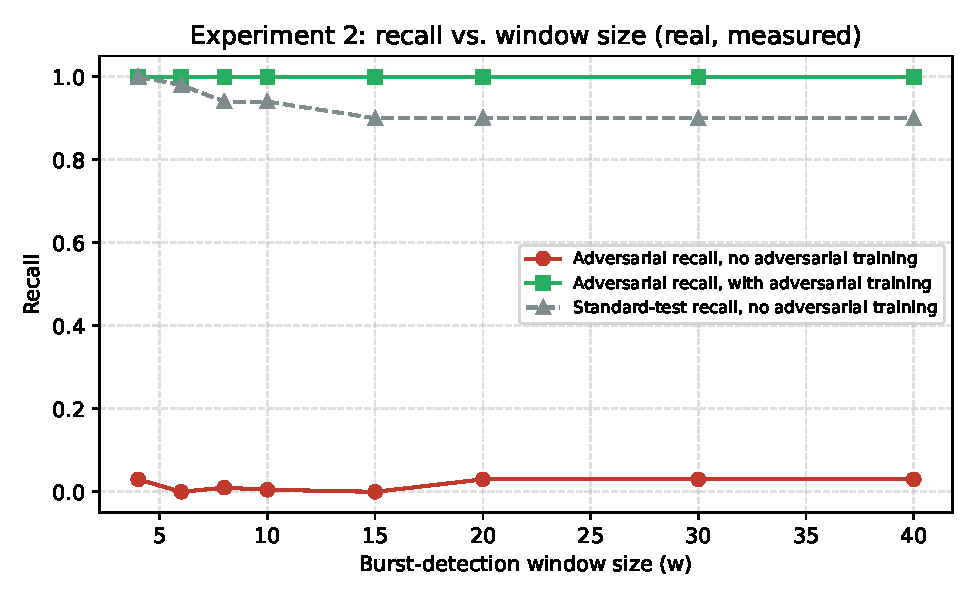
\includegraphics[width=0.85\linewidth]{figures/exp2_window_sweep.pdf}
\caption{Recall vs.\ burst-detection window size, actually measured at each of 8 window sizes (not illustrative). 200 Held-out low-and-slow adversarial sessions and a standard stratified test split, re-run per window size. Data: \texttt{results/exp2\_window\_sweep.json}, generator: \texttt{src/make\_figure3.py}}
\label{fig:sweep}
\end{figure}

\subsection{Experiment 3}

\begin{table}[h]
\centering
\begin{tabular}{@{}lc@{}}
\toprule
Metric & Value \\
\midrule
Events flagged & 1{,}500 / 50{,}000 (3.0\%) \\
Genuine anomalies among flagged & 97.4\% \\
Recall on true anomalies & 97.4\% \\
\bottomrule
\end{tabular}
\caption{Experiment 3 results.}
\end{table}

Because we set the contamination parameter to the true anomaly rate, the Isolation Forest's flagged count matches the true anomaly count almost exactly, a favorable setup we flag as a limitation.

Figure~\ref{fig:iso} plots the model's actual flagged points from this run (not a stylized illustration) along the two features that separate normal from anomalous behavior most visibly: hour of day and call rate. The four off-hour clusters correspond to the five off-hour values the generator draws anomalies from; the sparse red points inside the daytime cluster are the model's real false positives, normal-hour sessions with an unusually high call rate that get flagged anyway, which is the same conservative failure mode as Experiment 2 (Section 4.2): erring toward a false alarm rather than a miss.

\begin{figure}[h]
\centering
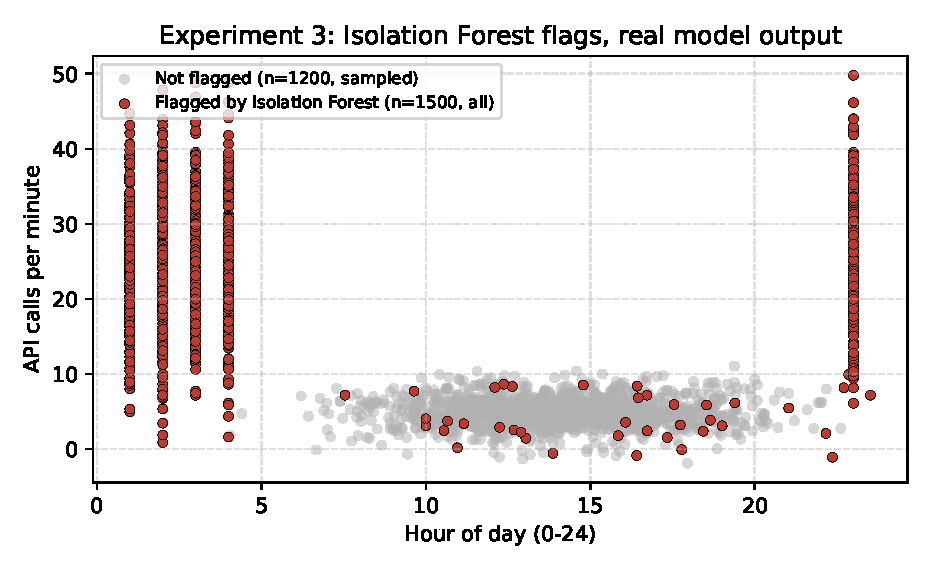
\includegraphics[width=0.8\linewidth]{figures/exp3_isolation_forest.pdf}
\caption{Real Isolation Forest output on the full 50{,}000-event dataset (flagged points shown in full; unflagged points subsampled to 1{,}200 for plot readability only, sampling does not affect the reported metrics). Data and flags are the direct, unmodified output of \texttt{src/exp3\_cloudtrail\_anomaly.py}; generator: \texttt{src/make\_figure2.py}}
\label{fig:iso}
\end{figure}

\section{Discussion}

The single biggest finding across all three experiments is that a model's synthetic-test performance and its real-world transfer are not the same thing and can even invert: in Experiment 1, the Random Forest beats the rule-based scanner by 23 points of accuracy on synthetic data (Table 1) but \emph{loses} to it by 42 points on real AWS-managed policies (Table 2), before a one-feature fix closes the gap. That inversion would be invisible without the external test, because the synthetic generator and the model's features were built by the same people with the same mental model of what ``risky'' looks like.

The Experiment 2 adversarial result makes a related point: the jump from a naive baseline to a working classifier came almost entirely from feature engineering, and that same feature engineering fails silently outside the conditions it was designed for: a wider detection window looks like it should help evasive attackers and simply doesn't, until training data itself contains the evasive pattern.

The false-positive patterns are also informative. In Experiment 1, the ambiguous PassRole+AssumeRole case is exactly what a human reviewer would also have to think carefully about. In Experiment 2, false positives concentrate in exactly the sessions designed to be genuinely ambiguous, which is a reasonable thing to flag for a human, not a failure.

\section{Limitations}

\begin{itemize}
\item \textbf{Real-world validation was only possible for Experiment 1, and only at modest scale.} 19 labeled real policies is enough to demonstrate a generalization failure and a fix, not enough for a precise, confidence-interval-backed real-world accuracy estimate. Experiments 2 and 3 have no equivalent real-data test: no public labeled dataset of real attacker API-call sessions exists for privacy/security reasons, and the one public raw CloudTrail log corpus we identified was not practical to obtain and parse within this project's scope.
\item \textbf{The remaining synthetic data (Experiments 2 and 3) still describes detector performance on data generated to match our own assumptions.} Real AWS environments have messier, more varied normal behavior.
\item \textbf{Isolation Forest's contamination parameter was set to the true rate.} In practice this is unknown in advance; that sensitivity is untested here.
\item \textbf{Adversarial evaluation is limited to one evasion strategy, and only for Experiment 2.} Experiment 1's real-world test is a generalization check, not an adversarial one. Experiment 3 was not adversarially tested at all.
\item \textbf{The Experiment 1 real-world fix was found and validated on the same 19 real policies used to report its improved accuracy}; a held-out, independently-sourced real-policy set is the natural next check.
\item \textbf{Scope is AWS-specific and limited to three tasks.}
\end{itemize}

\section{Future Work}

Scaling the Experiment 1 real-world validation to a larger, independently-sourced set of real IAM policies to get a tighter real-world accuracy estimate and check whether other features have the same narrow-service-list problem; obtaining and parsing a real, labeled CloudTrail log sample to give Experiment 3 an equivalent real-data check; replacing the sliding-window burst feature in Experiment 2 with an actual sequence model; testing Isolation Forest's sensitivity to a misestimated contamination rate; and a reinforcement-learning layer on top of Experiment 3's anomaly scores \cite{rlsecurity2025,rlincident2025}, grounded in this specific pipeline.

\section{Conclusion}

Three small, mostly-reproducible experiments show a consistent pattern, and it isn't the flattering one a purely synthetic evaluation would suggest. On synthetic data, simple rule-based detection gets you most of the way, and the remaining gap closes with feature engineering and a standard classifier. But the two places we tested past that comfortable synthetic setting both produced a negative result worth taking seriously: the Experiment 1 classifier's real-world accuracy collapses to worse than the simple rule engine it was supposed to beat, fixable only once we went looking with real data; and the Experiment 2 classifier's adversarial recall collapses to 3\% against an attacker who simply spreads out their actions, fixable only by training on that specific evasive pattern. Both of this paper's positive results needed a matching negative result, found by testing outside the conditions the model was built under, to be trustworthy. All code, data generators, the real-world validation script and data source, and full results are included so every number here can be checked rather than taken on faith.

\section*{Declarations}

\paragraph{Funding.} The authors did not receive support from any organization for the submitted work. No funding was received to assist with the preparation of this manuscript.

\paragraph{Competing interests.} The authors have no relevant financial or non-financial interests to disclose.

\paragraph{Ethics approval.} This study did not involve human participants, human data, or animals. All data used are either synthetically generated by the authors' own code or drawn from publicly published, non-personal AWS-managed IAM policy documents (Section 3.1). No ethics approval was required.

\paragraph{Consent to participate / Consent to publish.} Not applicable.

\paragraph{Data availability.} The synthetic data generators, the real-world validation script, and the result files (JSON) referenced in this paper are provided in the accompanying GitHub repository. A permanent, versioned archive can be added via Zenodo when available.

\paragraph{Code availability.} All source code (\texttt{src/}), including the three experiment scripts, the real-world validation script, and the figure-generation scripts, is available at the same repository and archive referenced above, under the MIT License.

\paragraph{Author contributions.} B.N. conceived the study, implemented the experiments and the real-world validation pipeline, and drafted the manuscript. N.A. contributed to experimental design and reviewed and revised the manuscript. Both authors read and approved the final manuscript.



\begin{thebibliography}{99}

\bibitem{shevrin2023} A. Shevrin, O. Peleg, et al., ``Detecting Multi-Step IAM Attacks in AWS Environments via Model Checking,'' \emph{32nd USENIX Security Symposium}, 2023.

\bibitem{vanede2022} T. van Ede, N. Khasuntsev, B. Steen, A. Continella, ``Detecting Anomalous Misconfigurations in AWS Identity and Access Management Policies,'' \emph{ACM Cloud Computing Security Workshop (CCSW)}, 2022.

\bibitem{wen2024} J. Wen, Z. Chen, F. Sarro, Z. Zhu, Y. Liu, H. Ping, S. Wang, ``LLM-Based Misconfiguration Detection for AWS Serverless Computing,'' arXiv:2411.00642, 2024.

\bibitem{rlsecurity2025} ``Adaptive Security Policy Management in Cloud Environments Using Reinforcement Learning,'' arXiv:2505.08837, 2025.

\bibitem{rlincident2025} ``Optimizing Cybersecurity Incident Response via Adaptive Reinforcement Learning,'' 2025.

\bibitem{owasp2023} OWASP Foundation, ``OWASP API Security Top 10,'' 2023.

\bibitem{nist800207} NIST Special Publication 800-207, ``Zero Trust Architecture,'' National Institute of Standards and Technology, 2020.

\bibitem{thales2024} Thales, ``2024 Cloud Security Study'' (as reported in Infosecurity Magazine, ``Cloud Breaches Impact Nearly Half of Organizations'').

\bibitem{ieeedataport} IEEE DataPort, ``Misconfiguration Detection Dataset for Cloud IAM and APIs.''

\bibitem{breiman2001} L. Breiman, ``Random Forests,'' \emph{Machine Learning}, vol. 45, no. 1, pp. 5--32, 2001.

\bibitem{liu2008} F. T. Liu, K. M. Ting, Z.-H. Zhou, ``Isolation Forest,'' \emph{Proc. IEEE 8th International Conference on Data Mining (ICDM)}, 2008, pp. 413--422.

\bibitem{rahman2023} A. Rahman, S. I. Shamim, D. B. Bose, R. Pandita, ``Security Misconfigurations in Open Source Kubernetes Manifests: An Empirical Study,'' \emph{ACM Transactions on Software Engineering and Methodology}, vol. 32, no. 4, pp. 1--36, 2023.

\bibitem{csa2024} Cloud Security Alliance, ``Top Threats to Cloud Computing 2024,'' 2024. \url{https://cloudsecurityalliance.org/artifacts/top-threats-to-cloud-computing-2024}

\bibitem{cloudsplaining} Salesforce, ``Cloudsplaining: An AWS IAM Security Assessment Tool,'' open-source software, Apache-2.0 License. \url{https://github.com/salesforce/cloudsplaining}

\bibitem{traildiscover} A. Alvarez, ``TrailDiscover: An Open, Incident-Linked Catalog of AWS CloudTrail Events,'' open-source dataset. \url{https://github.com/adanalvarez/TrailDiscover}

\end{thebibliography}

\end{document}
